\documentclass[aps,prl,twocolumn,superscriptaddress]{revtex4-1}

% the percent sign gives comments in Latex
% top line indicates this is for Physical Review, standard journal format,
% suitable for electronic submission of articles

% the line above is necessary to start any latex document.
% this is one variation that should work for most things.
% if you want double spaceing, use the following:
%
%\documentclass[prd,preprint,letterpaper]{revtex4}
%
% the "preprint" designation will make a wider line
% spacing, good for markup.
\usepackage{graphicx}  % this is the up-to-date package for all figures
\usepackage{amssymb}   % for math
\usepackage{verbatim}  % for the comment environment
\usepackage{color}
\usepackage{gensymb}
\usepackage{amsmath}

\usepackage[section]{placeins}

\usepackage{wrapfig}
\usepackage{hyperref}
\usepackage{titlesec}
\usepackage{amssymb}   % for math
\usepackage{verbatim}  % for the comment environment
\usepackage{color}
\usepackage[nodisplayskipstretch]{setspace}
\usepackage{amsmath}
\usepackage{blindtext}
%\usepackage[pdftex]{graphicx}
\usepackage[outdir=./]{epstopdf}
\usepackage[space]{grffile}
\usepackage{epsfig}
\usepackage[separate-uncertainty=true]{siunitx}
\usepackage{tikz}
\usepackage{pgfgantt}
\usepackage[english]{babel}
\usepackage[utf8]{inputenc}

\titlespacing*{\section}
{0pt}{1\baselineskip}{.5\baselineskip}

\titlespacing*{\subsection}
{0pt}{.5\baselineskip}{.3\baselineskip}



\bibliographystyle{apsrev}


% these are some custom control of the page size and margins
% \topmargin= 0.2in  % these 1st two may be needed for some computers
% \textheight=8.75in
%\textwidth=6.5in
%\oddsidemargin=0cm
%\evensidemargin=0cm

% this is where the actual document itself (rather than control statements) begins:

\begin{document}

% use a style that gives automatic headings
%\pagestyle{headings}



% the \title{} command generates a title.

% the \\ below is used to FORCE a line break in the middle of the sentence--
% otherwise latex computes it for you

\title{The Speed of Light}


\author{\textbf{Bryan Yamashiro}}
\author{Christina Nelson}
\author{Corey Mutnik}
\author{Daichi Hiramatsu}

\affiliation{Department of Physics \& Astronomy, \\
University of Hawaii at Manoa,\\
2505 Correa Rd, Honolulu, HI, 96822, USA}





	      % \section is used to start a new one with a heading
\begin{abstract}

This study measured the speed of light in an experiment apparatus. Instruments used to measure the speed of light included a light emitting dioide\,(LED), a photomultiplier tube\,(PMT), and fast pulse circuitry. Measured speeds of light were (3.06$\pm$0.16)$\times$10$^8$\,m/s and (3.13$\pm$0.50)$\times$10$^8$\,m/s for the pulse widths of 2\,ns and 40\,ns.




\end{abstract}

\maketitle    % this line is necessary to tell latex you are done with all
	      % of the stuff associated with the title, and now it can go
              % ahead and generate the title portion


\section{Background}

The method of measuring the speed of light used in this study is modeled after the Focault method, which used an apparatus containing sets of mirrors to project and measure light. The projected light reflects off a rotating mirror, to a fixed mirror, back to the rotating mirror, finally to a detector. The apparatus was optimized by Albert Michelson in the 1920s and experimentally measured the speed of light to an error of $\pm$4\,km/s\,\cite{1}. Apparatuses such as the Focault apparatus allow for measuring the speed of light in a laboratory.

 % the ~\cite{ } is how you link a reference in the text. The references
 % themselves are at the end.

% one or more lines of space between paragraphs determines them

\section{Apparatus}



The apparatus replicates the Focault instrument, but without the rotating reflector. Values of the speed of light were measured with different pulse widths. New components include the time-to-amplitude converter\,(TAC), Multi-Channel Analyzer\,(MCA), and the computer program\,(MAESTRO)\,\cite{2}. As the name suggests, the TAC converts the pulse time into decipherable amplitudes. The MCA takes the amplitude signal and distinguishes the counts across 2048 channels. MAESTRO compiles all amplitudes with corresponding channels and generates histograms and provides ASCII data. Components of the instrument are specified in figure 1.

\begin{figure}[h!]
  \begin{center}
\centerline{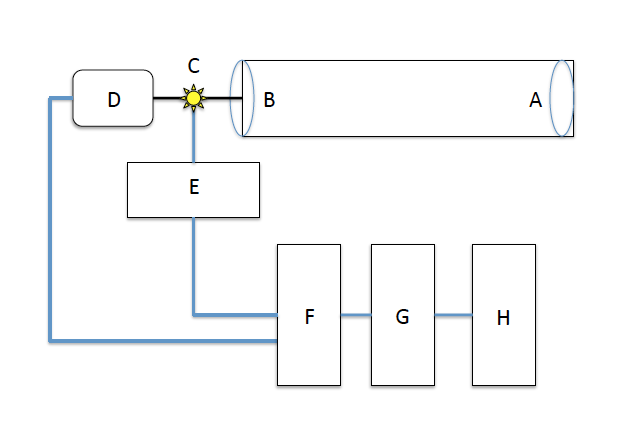
\includegraphics[width=3.in]{solapp.png}}
\caption{\it \small{A)\,Mirror, B)\,Fresnel Lens, C)\,LED Source, D)\,PMT, E)\,Pulser, F)\,TAC, G)\,MCA, H)\,MAESTRO.\,\cite{3}. \label{fig1}}}
  \end{center}
\end{figure}

\section{Procedure}


\begin{table}[htb!] 
\caption{\it Initial Apparatus Parameters}
		%table caption at the top is standard
\label{t1}   % labels are used to refer to this in the text
 \begin{center}   % center the table on the page
    \begin{tabular}{|c|c|c|} \hline   % tabular environment determines the

Pulse & Tube & MCA \\
Width & Length & Channels  \\
(ns)  & (in.) & (sec.)   \\ \hline \hline
    % the "~" character forces a non-breaking space--here is just makes the columns a bit wider
4 & 445.6$\pm$0.05 & 2048 \\ \hline
20 & 445.6$\pm$0.05  &  2048  \\ \hline

     \end{tabular}
  \end{center}
\end{table}

% you always need to end an environment { } you have started--just like in C

The experiment initiated with a LED emitting photons into the black enclosed tube\,\cite{3}. Photons initially traveled through a Fresnel lens, which in turn caused some backscatter of photons. These photons were detected first by the PMT at the early time, $t_1$. Photons that weren't backscattered pass through the Fresnel lens and were reflected off a mirror on the back of the enclosed tube. The reflected photons were then detected at a delayed time of $t_2$. The detected photons were then converted into electrons via photoelectric effect. Ultimately the pulses and the electrons were then converted into amplitude using the TAC and then split over multiple channels in a histogram compiled with MAESTRO.

\begin{figure}[h!]
  \begin{center}
\centerline{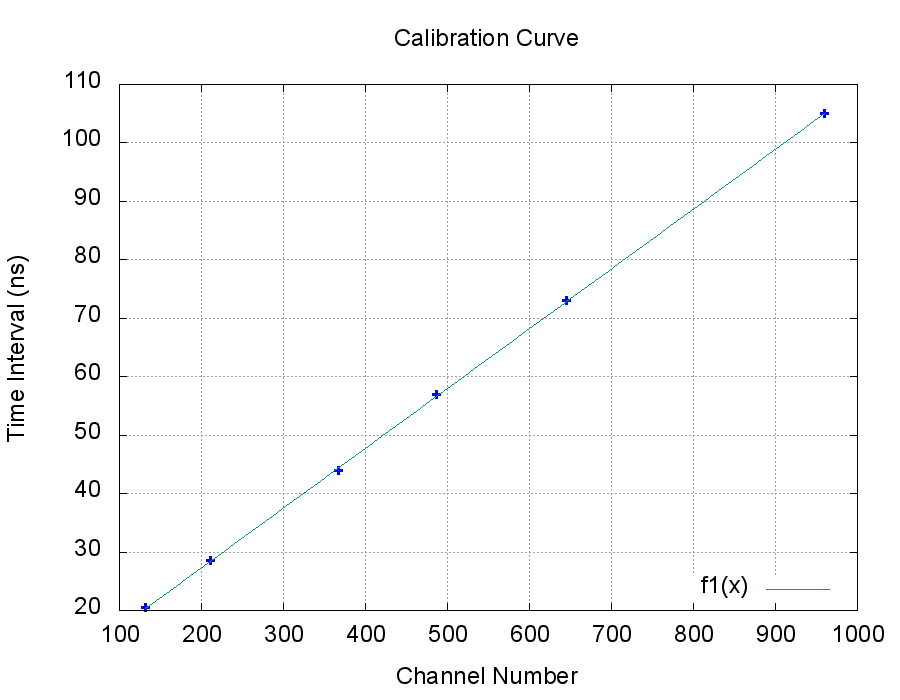
\includegraphics[width=3.5in]{calib.png}}
\caption{\it \small{Calibration curve of unique time intervals. The linear fit represents a correlation calibration between channel number and time. \label{fig1}}}
  \end{center}
\end{figure}

A calibration curve was compiled to represent the time interval\,($\Delta$t) versus the MCA channel number for six unique time intervals for a linear fit. A linear fit was used to convert the channel numbers for the difference in time between the two-histogram peaks generated by MAESTRO. Resulting time for the peak difference was utilized along with the measured enclosed tube length to determine an experimental estimate of the speed of light.
\\
\indent Two trials of different pulse widths were conducted, including 2\,ns and 40\,ns. Nothing except the pulse widths were manipulated during this study to represent a fixed system with one changing parameter.





\section{Calculation of Results and Errors}

\begin{equation}
c = \frac{2L}{\Delta t}
\end{equation}

The measured speed of light, $c$, was calculated using equation 1. Input parameters are shown in table 1. MAESTRO provided an ASCII data file that was then plotted, portrayed in figure 3 and 4. Both figures show two peaks for both the 2\,ns and 40\,ns.

\begin{figure}[h!]
  \begin{center}
\centerline{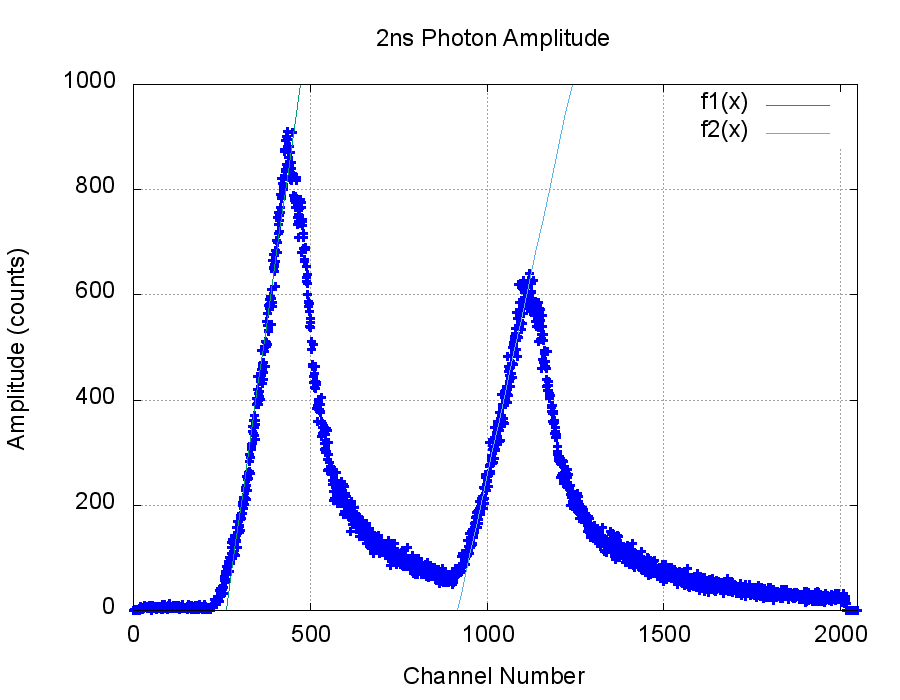
\includegraphics[width=3.5in]{solgraph2.png}}
\caption{\it \small{2\,ns pulse width photon amplitude. \label{fig1}}}
  \end{center}
\end{figure}

\begin{figure}[h!]
  \begin{center}
\centerline{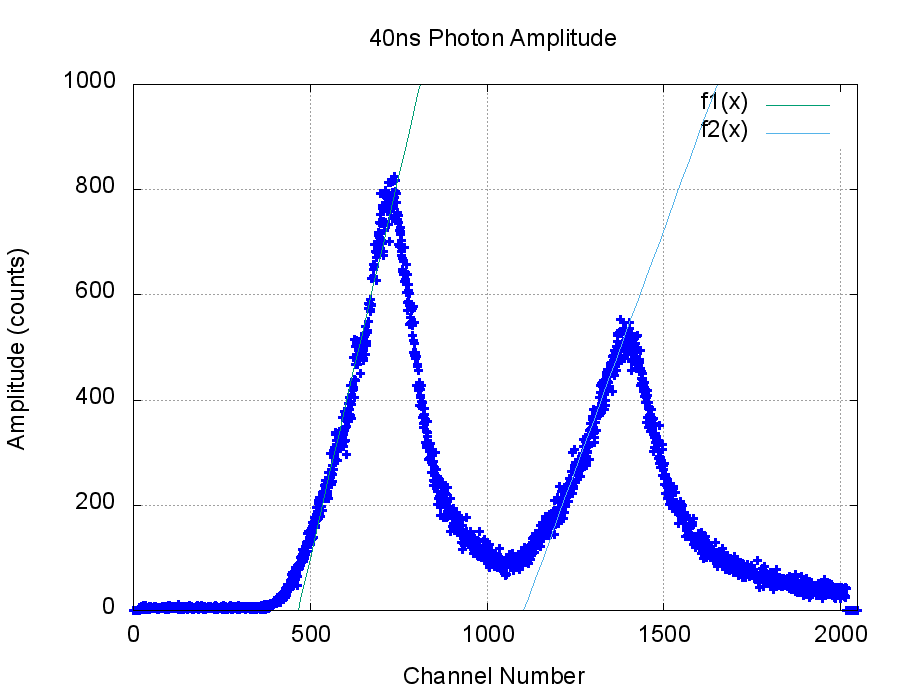
\includegraphics[width=3.5in]{solgraph40.png}}
\caption{\it \small{40\,ns pulse width photon amplitude. \label{fig1}}}
  \end{center}
\end{figure}

The two peaks correlate to the time of initial detection of reflected photons off the Fresnel lens, and the final detection of photons from the mirror at the back of the tube. Linear regressions were fit to the ascending slopes of the two peaks. Differences are taken from the x-intercepts of the fits for the difference in channel numbers. The channel difference is calibrated with the calibration curve to output a time difference. Initial length of the tube and time differences resulted in a measured speed of light.
\\
\indent The two speed of light experimental measurements are (3.06$\pm$0.16)$\times$10$^8$\,m/s and (3.13$\pm$0.50)$\times$10$^8$\,m/s for the 2\,ns and 40\,ns respectively. Compared to the true speed of light, 299,792,458\,m/s, the two experimental speeds are within the statistical error.


\section{Discussion}

Measured speeds of light were determined to be similar to the theoretical speed of light. The double linear fits provided channel differences leading to a stable estimate of the time difference. Length of the tube was affected by extra slack in the measuring tape. Both measurements of speed of light were larger than the theoretical value and the slack could have factored into the calculation of equation 1.


% the following \setlength is to force the bibliography to have no
% paragraph indentations.Can use vairous units--cm are used here.
\setlength{\parindent}{0cm}

\begin{thebibliography}{99}  % the trailing 99 controls some obscure format--just use

\bibitem{1} McFarland, Kevin. "Speed of Light Demonstration by the Foucault Method." University of Rochester. Web. 5 Nov. 2015.     % {\em } for emphasis, \textbf{ } for boldface

\bibitem{2} "Multichannel Analyzer (MCA) Application Software." Nuclear Applications Software|ORTEC Scientific Equipment. ORTEC. Web. 5 Nov. 2015.

\bibitem{3} THE SPEED OF LIGHT. (n.d.). Retrieved November 4, 2015, from \url{http://www.phys.hawaii.edu/~teb/phys480l/SpeedOfLight.txt}




\end{thebibliography}





\end{document}

